\documentclass[11pt]{article}

\usepackage[margin=1in]{geometry}
\usepackage{amsmath,amssymb,amsthm,mathtools}
\usepackage{graphicx}
\usepackage{booktabs}
\usepackage{multirow}
\usepackage{hyperref}
\usepackage{caption}
\usepackage{microtype}
\usepackage{enumitem}
\usepackage{authblk}
\usepackage{xcolor}
\usepackage{natbib}

\hypersetup{
  colorlinks=true,
  linkcolor=blue!50!black,
  citecolor=blue!50!black,
  urlcolor=blue!60!black,
}

\newcommand{\R}{\mathbb{R}}
\newcommand{\E}{\mathbb{E}}
\newcommand{\Var}{\mathrm{Var}}
\newcommand{\Cov}{\mathrm{Cov}}
\newcommand{\diag}{\mathrm{diag}}
\newcommand{\trace}{\mathrm{tr}}
\newcommand{\CTX}{[\mathrm{CTX}]}
\newcommand{\Sig}{\boldsymbol{\Sigma}}
\newcommand{\bmu}{\boldsymbol{\mu}}
\newcommand{\br}{\mathbf{r}}
\newcommand{\bw}{\mathbf{w}}
\newcommand{\bL}{\mathbf{L}}
\newcommand{\bB}{\mathbf{B}}
\newcommand{\bF}{\mathbf{F}}
\newcommand{\bD}{\mathbf{D}}
\newcommand{\softplus}{\mathrm{softplus}}

\DeclareMathOperator*{\argmin}{arg\,min}
\DeclareMathOperator*{\argmax}{arg\,max}

\title{\bfseries Regime-Aware Dynamic Asset Allocation via a Cross-Asset Transformer with Factor-Structured Covariance Forecasting}

\author{Tyler Pellek\thanks{Princeton University. Correspondence: \href{mailto:tp5523@princeton.edu}{\texttt{tp5523@princeton.edu}}.}}

\date{May 2026}

\begin{document}
\maketitle

\begin{abstract}
\noindent
This paper specifies and evaluates a portfolio strategy that combines a
Cross-Asset Transformer with a constrained mean--variance optimizer on a
fixed long-only universe of sixteen U.S.\ mega-capitalization technology
equities. At each weekly rebalance, the model produces a forward
covariance matrix $\Sig \in \R^{N \times N}$ parameterized through a
rank-$k$ factor decomposition $\Sig = \bB \bF \bB^\top + \bD$, where the
regime-conditional factor covariance $\bF$ is predicted from a global
context token carrying Hidden Markov Model regime posteriors and
macroeconomic features. The model is trained per fold under a Gaussian
negative log-likelihood objective on five-day forward cumulative log
returns, with warm-start fine-tuning across walk-forward folds. The
model-implied covariance is blended with a rolling sample covariance at
$\alpha = 0.7$, and the resulting estimate is passed to a long-only
mean--variance optimizer with an explicit weekly volatility cap. Across
an eighteen-fold walk-forward backtest covering 2008--2024 (4,417
out-of-sample trading days spanning the global financial crisis, the
COVID-19 shock, the 2022 bear market, and the 2023 regional banking
crisis), the strategy attains an annualized Sharpe ratio of $1.21$, a
maximum drawdown of $-25.06\%$, and a Calmar ratio of $0.94$, exceeding
the corresponding metrics of seven classical portfolio-construction
baselines---equal-weight, inverse-volatility, equal risk-contribution
risk-parity, minimum-variance, sample-statistics mean--variance,
long-only tangency, and SPY---on the same out-of-sample window. An
ablation study of eighteen perturbations of the configuration is reported
in the appendix; all eighteen reduce out-of-sample Sharpe ratio.
\end{abstract}

\noindent\textbf{Keywords:} Portfolio optimization; Transformer; Walk-forward
evaluation; Hidden Markov model; Covariance forecasting; Factor model.

% ============================================================
\section{Introduction}\label{sec:intro}
% ============================================================

The Markowitz mean--variance framework \citep{markowitz1952} reduces
asset allocation to a pair of inputs---expected returns $\bmu$ and a
covariance matrix $\Sig$---and a deterministic convex optimization step.
Two empirical regularities of asset returns violate the framework's
implicit assumptions: conditional variance is auto-correlated
\citep{bollerslev1986}, and pairwise correlations rise toward unity
during periods of broad-market stress \citep{longin2001}. The first
implies that $\Sig$ is not stationary; the second implies that the
diversification benefit a static covariance matrix attributes to a
portfolio is largest precisely when it is least real.

Existing responses parameterize the conditional dynamics. Multivariate
GARCH \citep{engle2002,bauwens2006} models $\Sig_t$ recursively from
residuals; risk-only methods such as minimum-variance and equal
risk-contribution \citep{maillard2010} dispense with $\bmu$;
regime-switching models \citep{hamilton1989,ang2002} introduce latent
discrete states to capture qualitative shifts in joint behavior;
shrinkage estimators \citep{ledoit2004} blend the sample covariance
toward a structured target. Recent neural-network approaches apply
sequence models to multivariate return prediction
\citep{li2021,wang2022}, sometimes combined with differentiable
optimization layers \citep{donti2017,butler2023}.

This paper synthesizes three of these ideas. (1) Each asset is encoded
as a token in a self-attention sequence prepended by a global $\CTX$
token carrying macroeconomic and regime-detection features.
(2) The covariance head adopts a rank-$k$ factor parameterization
\(
\Sig = \bB \bF \bB^\top + \bD
\)
in which the factor covariance $\bF$ is regime-conditional through the
$\CTX$ embedding; this reduces the head's free parameter count from
$N(N{+}1)/2$ to $Nk + k(k{+}1)/2 + N$ and imposes a Fama--French-style
inductive bias \citep{fama1993}. (3) Training is organized as expanding
walk-forward folds with warm-start fine-tuning across boundaries,
preserving the network's representation of prior regimes.

The primary contribution is a complete specification and out-of-sample
evaluation of this architecture against seven classical baselines on a
seventeen-year walk-forward backtest. The secondary contribution is a
systematic ablation: eighteen single-knob perturbations of the
production configuration are evaluated and all are found to reduce
out-of-sample Sharpe ratio. Section~\ref{sec:method} specifies the
architecture, training procedure, and portfolio-construction step.
Section~\ref{sec:experiments} describes the dataset, walk-forward
protocol, baselines, and metrics. Section~\ref{sec:results} reports
performance. Section~\ref{sec:discussion} discusses interpretation and
limitations. Section~\ref{sec:conclusion} concludes.
Appendix~\ref{app:ablation} reports the ablation;
Appendix~\ref{app:hyperparams} lists hyperparameters.

% ============================================================
\section{Methodology}\label{sec:method}
% ============================================================

\subsection{Setup}\label{sec:setup}

Let $N$ denote the number of tradable assets and $W$ the lookback
window in trading days. Daily log returns are $r_{t,i} =
\log(P_{t,i}/P_{t-1,i})$ and the cross-section is $\br_t \in \R^N$. At
rebalance date $t$ the model receives features from the trailing $W$
days plus a context vector and outputs $(\bmu_t, \Sig_t)$ for the
forward $h$-day horizon. Portfolio weights $\bw_t \in \R^N$ are
selected by solving the convex program in
Section~\ref{sec:portfolio}. A binary mask $\mathbf{m}_t \in \{0,1\}^N$
indicates each asset's tradability at $t$ (an asset becomes active once
it has $W$ valid prior observations, handling staggered IPO dates);
attention is masked accordingly and inactive assets are excluded from
the optimization.

\subsection{Cross-Asset Transformer}\label{sec:architecture}

The model operates on a sequence of $N{+}1$ tokens: a global context
token at position $0$ and one asset token at each of positions
$1,\ldots,N$.

\paragraph{Context token features.} The $\CTX$ token's raw vector
concatenates (i) the posterior probabilities of a $K$-state Gaussian
Hidden Markov Model fit on a low-dimensional aggregate market signal
(daily S\&P~500 log return and log VIX), and (ii) macroeconomic features
including the VIX level and $W$-day log change, the $W$-day S\&P~500
return, the 10-year Treasury yield level and $W$-day change, the
$W$-day returns of the dollar index and crude oil, an HYG/TLT credit
spread proxy, and the 10-year-minus-3-month and 30-year-minus-10-year
yield-curve term spreads. The HMM is re-fit at the start of each
walk-forward fold using only data available up to that fold's training
cutoff and is held fixed during the corresponding test window.

\paragraph{Asset token features.} The raw vector for asset $i$ at date
$t$ concatenates: (i) the $W$ trailing daily log returns; (ii) the
rolling $W$-day standard deviation of returns; (iii) the previous-period
portfolio weight $w_{t-1,i}$; and (iv) four normalized OHLCV-derived
features---rolling 5-day means of intraday range $(H-L)/C$, intraday
return $(C-O)/O$, overnight gap $(O - C_{\text{prev}})/C_{\text{prev}}$,
and a 60-day rolling $z$-score of trading volume. Each of the four
OHLCV features is rolling-$z$-scored over a 252-day window so all
features share comparable numerical scale.

\paragraph{Projection and self-attention.} Two linear projections embed
the raw $\CTX$ features $\mathbf{c}_t \in \R^{d_c}$ and the raw asset
features $\mathbf{a}_{t,i} \in \R^{d_a}$ into a common dimension
$d_{\text{model}}$, with learned positional embeddings
$\mathbf{p}_{\CTX}, \mathbf{p}_i \in \R^{d_{\text{model}}}$:
\begin{align}
\tilde{\mathbf{c}}_t &= W_{\CTX}\, \mathbf{c}_t + \mathbf{p}_{\CTX}, &
\tilde{\mathbf{a}}_{t,i} &= W_{\text{asset}}\, \mathbf{a}_{t,i} + \mathbf{p}_i.
\end{align}
The sequence $X_t = [\tilde{\mathbf{c}}_t,\, \tilde{\mathbf{a}}_{t,1},
\ldots,\tilde{\mathbf{a}}_{t,N}] \in \R^{(N+1)\times d_{\text{model}}}$
is passed through $L$ pre-LayerNorm Transformer blocks
\citep{vaswani2017,xiong2020} with multi-head self-attention and a
position-wise feed-forward network. The attention masks inactive assets
at every layer.

\paragraph{What is learned.} The projection matrices $W_{\CTX} \in
\R^{d_{\text{model}}\times d_c}$ and $W_{\text{asset}} \in
\R^{d_{\text{model}}\times d_a}$, the positional embeddings
$\mathbf{p}_{\CTX}$ and $\{\mathbf{p}_i\}_{i=1}^{N}$, and every weight
in the transformer blocks and output heads are jointly learned
parameters trained end-to-end under the likelihood objective of
\eqref{eq:nll}. The total parameter count of the production model is
approximately $1.8 \times 10^{6}$. A single asset-projection matrix
$W_{\text{asset}}$ is shared across all $N$ asset tokens: the model
treats every asset's raw feature vector through the same linear map,
and per-asset identity enters solely through the learned positional
embedding $\mathbf{p}_i$. This factorization is what makes the
architecture a genuine cross-asset model rather than $N$ parallel
single-asset models. The HMM parameters, by contrast, are fit
separately by Baum-Welch on the macro signal and are \emph{not} in
the gradient graph: the transformer treats the HMM's three regime
posteriors as fixed inputs at each snapshot. Macroeconomic feature
definitions and OHLCV $z$-score normalization statistics are
deterministic functions of the training-window data and are likewise
held fixed at inference. Warm-start fine-tuning
(\S\ref{sec:walkforward}) carries the learned weights, including the
input embeddings, across all eighteen walk-forward folds.

\subsection{Factor-structured covariance head}\label{sec:factor_head}

A full lower-triangular Cholesky head would predict $N(N{+}1)/2 = 136$
free entries per snapshot at $N=16$, against approximately 500--2,500
training snapshots per walk-forward fold. To reduce the parameter count
and impose a financial-economics inductive bias, the head produces a
rank-$k$ factor decomposition with $k = 4$:
\begin{equation}
\Sig_t = \bB_t \bF_t \bB_t^\top + \bD_t.
\label{eq:factor}
\end{equation}

\paragraph{Loadings.} A linear head maps each asset embedding
$\mathbf{h}_{t,i}$ to a $k$-vector $\bB_{t,i} = W_B\, \mathbf{h}_{t,i}$;
$\bB_t \in \R^{N\times k}$ is the row-stack.

\paragraph{Idiosyncratic variance.} A scalar head produces
\begin{equation}
d_{t,i} = \softplus\bigl(W_d\, \mathbf{h}_{t,i} - c\bigr) + \sigma_{\min},
\qquad
\bD_t = \diag\bigl(d_{t,1}^2,\ldots,d_{t,N}^2\bigr).
\end{equation}
The shift $c = 4$ initializes $d_{t,i}$ near $0.02$, matching the
empirical weekly standard deviation of mega-cap U.S.\ equities;
$\sigma_{\min} = 10^{-2}$ enforces a positive floor.

\paragraph{Regime-conditional factor covariance.} A linear head on the
$\CTX$ embedding $\mathbf{h}_{t,0}$ produces the $k(k{+}1)/2$
lower-triangular entries of a Cholesky factor $\bF_t^{1/2}$ with positive
diagonal enforced via softplus, and $\bF_t = \bF_t^{1/2}(\bF_t^{1/2})^\top$.
Since $\bF_t$ is derived from the $\CTX$ embedding, it inherits the
regime conditioning carried by the HMM posteriors and macro features.

\paragraph{Cholesky for downstream operations.} A small jitter is added
and the lower-triangular Cholesky factor is computed via differentiable
decomposition, $\bL_t = \mathrm{chol}(\Sig_t + \epsilon I)$, for use in
the training loss.

\paragraph{Mean head.} A two-layer MLP maps each asset embedding to a
scalar $\mu_{t,i}$. The mean head is trained jointly with the
covariance head under the likelihood objective; at inference, however,
$\bmu_t$ is not used---see Section~\ref{sec:training_use_mu}.

\subsection{Training objective}\label{sec:loss}

Define $\br_{t,t+h} = \sum_{s=1}^{h}\br_{t+s}$ and let $\mathcal{A}_t$
denote the assets active at both $t$ and $t{+}h$. The per-snapshot
loss is the per-active-asset normalized Gaussian negative
log-likelihood evaluated on the active sub-block:
\begin{equation}
\mathcal{L}_t = \frac{1}{|\mathcal{A}_t|}\cdot
\frac{1}{2}\!\left[
|\mathcal{A}_t|\log(2\pi)
+ \log\det \Sig_t^{\mathcal{A}}
+ (\br_{t,t+h}^{\mathcal{A}} - \bmu_t^{\mathcal{A}})^\top
  (\Sig_t^{\mathcal{A}})^{-1}
  (\br_{t,t+h}^{\mathcal{A}} - \bmu_t^{\mathcal{A}})
\right].
\label{eq:nll}
\end{equation}
The Cholesky decomposition of $\Sig_t^{\mathcal{A}}$ supplies the
log-determinant as $2\sum_{i\in\mathcal{A}_t}\log L_{ii}$ and the
quadratic form via two triangular solves. Training uses AdamW with
cosine annealing, gradient clipping at $1.0$, and early stopping with
six-epoch patience and best-validation weight restoration.

\subsection{Walk-forward training with warm-start fine-tuning}\label{sec:walkforward}

Training is organized as a sequence of expanding-window folds. Fold $f$
trains on $[t_{\text{start}},\, t_f^{\text{train}}]$ and is evaluated
on $(t_f^{\text{train}},\, t_{f+1}^{\text{train}}]$, where
$t_f^{\text{train}} = t_{f-1}^{\text{train}} + \Delta_{\text{test}}$
with $\Delta_{\text{test}} = 252$ business days. Fold $0$ is initialized
from random weights; fold $f$ for $f\geq 1$ is initialized from the
state dictionary of fold $f{-}1$, with the base learning rate scaled by
$\eta_{\text{warm}} = 0.5$. The HMM is re-fit at the start of each fold
on data available up to $t_f^{\text{train}}$. Warm-start fine-tuning
preserves the network's representation of historical regimes; a cold
initialization for each fold reduces out-of-sample Sharpe ratio from
$1.02$ to $0.27$ on an otherwise-identical configuration
(Appendix~\ref{app:ablation}, Table~\ref{tab:ablation_arch}).

\subsection{Inference-time covariance shrinkage}\label{sec:shrinkage}

At each rebalance the model-implied covariance is convex-blended with a
horizon-scaled rolling sample covariance:
\begin{equation}
\Sig_t^{\text{final}} = \alpha\,\Sig_t^{\text{model}} + (1-\alpha)\,\Sig_t^{\text{sample}},
\quad
\Sig_t^{\text{sample}} = h\cdot \widehat{\Cov}\bigl(\br_{t-W+1},\ldots,\br_t\bigr).
\label{eq:shrinkage}
\end{equation}
Blending in covariance space preserves positive semidefiniteness. The
production value $\alpha = 0.7$ assigns 70\% weight to the model.
This is structurally analogous to Ledoit--Wolf shrinkage
\citep{ledoit2004} with the model's prediction as the structured
target.

\subsection{Portfolio construction}\label{sec:portfolio}

The expected-return vector fed to the optimizer is the rolling $W$-day
sample mean scaled to the forward horizon (see
Section~\ref{sec:training_use_mu}):
\begin{equation}
\bmu_t^{\text{opt}} = \frac{h}{W}\sum_{s=t-W+1}^{t} \br_s.
\label{eq:mu_sample}
\end{equation}
The convex program is
\begin{equation}
\begin{aligned}
\bw_t^\star =\ \argmin_{\bw \in \R^N}\quad
& -\bmu_t^{\text{opt}\,\top}\bw
+ \tfrac{\gamma}{2}\,\bw^\top \Sig_t^{\text{final}} \bw
+ \lambda_{\text{TO}}\,\|\bw - \bw_{t-1}\|_1\\
\text{subject to}\quad
& \mathbf{1}^\top \bw = 1,
\quad
0 \leq w_i \leq w_{\max} \text{ for } i\in\mathcal{A}_t,
\quad
w_i = 0 \text{ for } i\notin\mathcal{A}_t,\\
& \sqrt{\bw^\top \Sig_t^{\text{final}} \bw} \leq \bar{\sigma},
\end{aligned}
\label{eq:opt}
\end{equation}
with $\gamma$ a risk-aversion parameter, $\lambda_{\text{TO}}$ a
turnover penalty, $w_{\max}$ a concentration cap, and $\bar{\sigma}$ a
weekly volatility cap expressed as a second-order cone via the Cholesky
factor of $\Sig_t^{\text{final}}$. The program is solved with Clarabel
\citep{clarabel} through CVXPY \citep{cvxpy2016}.

\paragraph{Rationale for the sample-mean signal.}\label{sec:training_use_mu}
The model's mean head $\bmu_t$ is trained jointly with $\Sig_t$ under
\eqref{eq:nll} but is not used at inference. Substituting $\bmu_t$, a
12-1 Jegadeesh--Titman momentum signal, blended momentum variants, or
a 63-day vol-normalized Sharpe momentum reduces out-of-sample Sharpe
ratio in all cases (Appendix~\ref{app:ablation},
Table~\ref{tab:ablation_signal}). A consistent interpretation is that
the model's $\Sig_t$ supplies the regime-conditional information used
for portfolio construction, while the sample-mean signal provides a
smoothly varying fully-invested anchor that does not conflict with
$\Sig_t$.

% ============================================================
\section{Experimental setup}\label{sec:experiments}
% ============================================================

\subsection{Universe and data}

The universe is sixteen U.S.\ mega-capitalization technology equities:
AAPL, MSFT, GOOGL, AMZN, FB,\footnote{The underlying dataset is a
snapshot dated April 2020 in which the ticker FB refers to the entity
later renamed META.} NFLX, NVDA, TSLA, ADBE, CRM, ORCL, INTC, CSCO,
QCOM, IBM, TXN. Daily OHLCV bars from each listing date through April
2020 are obtained from the Kaggle dataset
\texttt{jacksoncrow/stock-market-dataset}; the series are extended
through December 2024 via Yahoo Finance \citep{yfinance}, anchored on
the April 2020 close ratio. TSLA enters in 2010-06 and FB in 2012-05;
the availability mask encodes their entry.

\subsection{Walk-forward protocol}\label{sec:wf}

The backtest runs from 2008-01-02 through 2024-12-30 with rebalances
every fifth trading day. The initial training cutoff is 2007-12-31 and
the fold test length is $252$ business days, producing eighteen folds.
Fold 1 tests through December 2008 (the 2008 crisis fully out-of-sample);
fold 12 tests through July 2020 (containing the March 2020 COVID-19
shock); fold 14 tests through June 2022 (the 2022 bear market); fold 15
tests through June 2023 (the regional banking crisis); fold 18 tests
through December 2024. The total is $4{,}417$ out-of-sample trading days
and $897$ rebalance decisions.

\subsection{Baselines}\label{sec:baselines}

Seven baselines are evaluated on the same calendar under the same
long-only fully-invested constraints ($\mathbf{1}^\top\bw = 1$,
$0 \leq w_i \leq w_{\max}$):
(1) \emph{equal weight}, $w_i = 1/|\mathcal{A}_t|$;
(2) \emph{inverse volatility}, $w_i \propto 1/\hat{\sigma}_i$ from
rolling 60-day std;
(3) \emph{equal risk-contribution risk-parity} \citep{maillard2010}
under rolling sample covariance;
(4) \emph{minimum variance}, $\argmin \bw^\top \Sig^{\text{sample}} \bw$;
(5) \emph{Markowitz mean--variance} with rolling sample $\bmu$ and
$\Sig$;
(6) \emph{long-only maximum Sharpe (tangency)}, solved via the
standard rotation;
(7) \emph{SPDR S\&P~500 ETF (SPY)} as a passive benchmark.

\subsection{Evaluation metrics}

Standard metrics on daily returns $r_t^P$: CAGR $= (\prod_t(1+r_t^P))^{252/N} - 1$;
annualized volatility $\hat{\sigma}_P = \mathrm{std}(r_t^P)\sqrt{252}$;
Sharpe $= (\overline{r^P}/\mathrm{std}(r_t^P))\sqrt{252}$;
maximum drawdown $\mathrm{MaxDD} = \min_t (E_t - \max_{s\leq t}E_s)/\max_{s\leq t}E_s$
with $E_t = \prod_{s\leq t}(1+r_s^P)$;
Calmar $= \mathrm{CAGR}/|\mathrm{MaxDD}|$;
Sortino $= (\overline{r^P}/\sqrt{\overline{\min(r_t^P,0)^2}})\sqrt{252}$.
Annualized $\alpha$ and $\beta$ relative to SPY are computed by OLS on
daily returns over the common overlap window.

% ============================================================
\section{Results}\label{sec:results}
% ============================================================

\subsection{Headline metrics}\label{sec:headline}

Table~\ref{tab:headline} reports out-of-sample metrics over the
$4{,}417$-day window.

\begin{table}[h]
\centering
\caption{Out-of-sample performance, 2008-01 to 2024-12 (18 walk-forward folds, 4{,}417 OOS days).}
\label{tab:headline}
\small
\begin{tabular}{lrrrrrrr}
\toprule
Strategy & CAGR & Vol & Sharpe & MaxDD & Calmar & $\beta$ & $\alpha_{\text{ann}}$ \\
\midrule
\textbf{Strategy (production)} & \textbf{0.2356} & \textbf{0.1901} & \textbf{1.21} & \textbf{$-$0.251} & \textbf{0.94} & \textbf{0.51} & \textbf{0.1759} \\
Max-Sharpe (tangency)          & 0.2698 & 0.2691 & 1.02 & $-$0.576 & 0.47 & --   & --     \\
Equal weight                   & 0.2226 & 0.2403 & 0.96 & $-$0.514 & 0.43 & 1.09 & 0.107  \\
Inverse volatility             & 0.2012 & 0.2312 & 0.91 & $-$0.502 & 0.40 & 1.06 & 0.090  \\
Risk parity (ERC)              & 0.1732 & 0.2085 & 0.87 & $-$0.499 & 0.35 & --   & --     \\
Min variance                   & 0.1543 & 0.1965 & 0.83 & $-$0.475 & 0.33 & --   & --     \\
Markowitz MV (sample stats)    & 0.1263 & 0.1956 & 0.71 & $-$0.389 & 0.32 & --   & --     \\
SPY benchmark                  & 0.1034 & 0.1903 & 0.61 & $-$0.552 & 0.19 & 1.00 & 0.000  \\
\bottomrule
\end{tabular}
\end{table}

The production strategy attains the highest Sharpe ratio, the highest
Calmar ratio, and the smallest maximum drawdown among the strategies
evaluated, and the lowest beta to SPY among the strategies with a
defined beta.

\subsection{Equity curves and drawdown}

\begin{figure}[h]
\centering
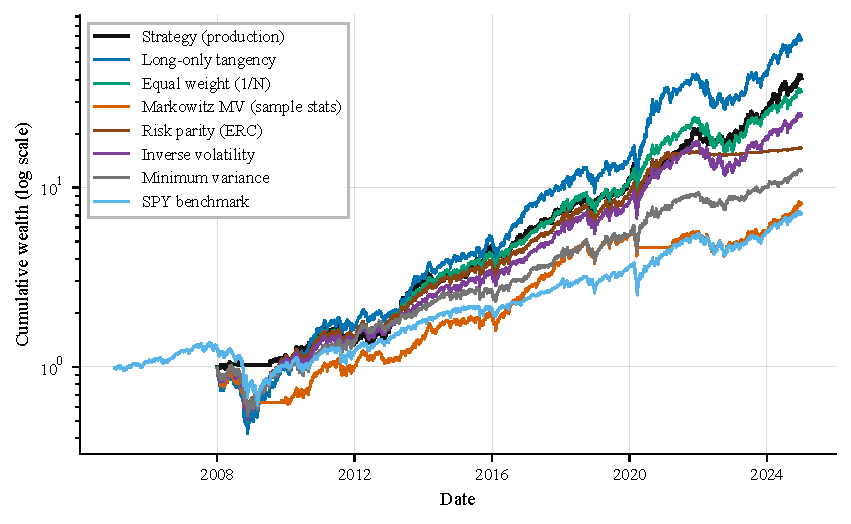
\includegraphics[width=\linewidth]{fig_equity.pdf}
\caption{Out-of-sample equity curves on a logarithmic vertical axis,
start $= \$1$. The production strategy is plotted in black against the
seven baselines. The long-only tangency baseline
(\texttt{max\_sharpe}, blue) terminates at higher cumulative wealth
but realizes a $-57.6\%$ maximum drawdown versus the strategy's
$-25.1\%$ (cf.~Figure~\ref{fig:drawdown} and
Table~\ref{tab:headline}).}
\label{fig:equity}
\end{figure}

\begin{figure}[h]
\centering
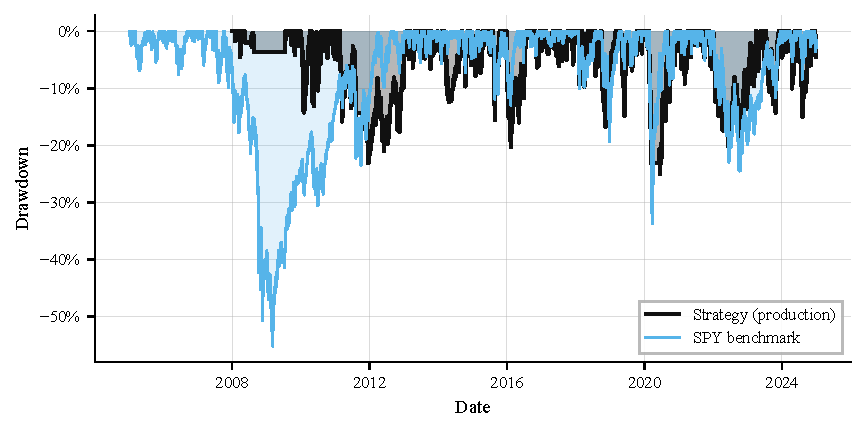
\includegraphics[width=\linewidth]{fig_drawdown.pdf}
\caption{Drawdown profiles. The strategy's maximum drawdown of
$-25.06\%$ occurs on 2020-06-11 during the COVID-19 dislocation,
against SPY's peak-to-trough drawdown of $-55.19\%$ over the sample.
The strategy traverses the 2008 global financial crisis with a
maximum drawdown of only $-4.5\%$.}
\label{fig:drawdown}
\end{figure}

Figure~\ref{fig:equity} shows the log-scale equity curves. The
long-only tangency baseline (\texttt{max\_sharpe}) terminates at a
higher cumulative wealth than the production strategy ($\$66.9$ versus
$\$40.8$ on a $\$1$ start), but does so with a maximum drawdown of
$-57.6\%$ and a Sharpe ratio of $1.02$, against the production
strategy's $-25.1\%$ and $1.21$. The production strategy is the
risk-adjusted leader; the long-only tangency baseline is the
unconditional-return leader. Figure~\ref{fig:drawdown} isolates the
strategy's drawdown profile against SPY. Secondary drawdown episodes
in the strategy fall in the $-15\%$ to $-22\%$ range and correspond to
the August 2011 sovereign-debt sell-off, the fourth-quarter 2018
drawdown, and the late-2022 bear market.

\subsection{Risk-adjusted ranking}

\begin{figure}[h]
\centering
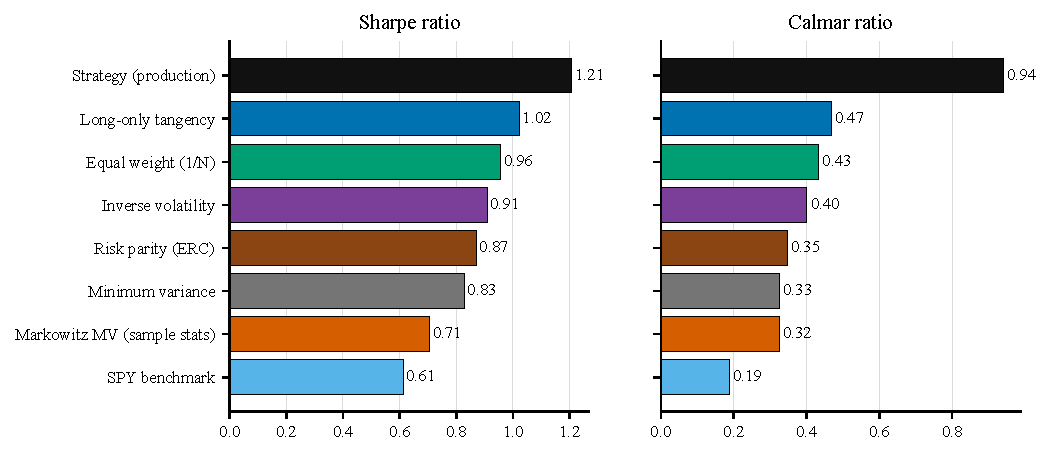
\includegraphics[width=\linewidth]{fig_metrics.pdf}
\caption{Cross-strategy comparison on Sharpe (left panel) and Calmar
(right panel) over the common out-of-sample window.}
\label{fig:metrics}
\end{figure}

Figure~\ref{fig:metrics} ranks strategies on Sharpe and Calmar. The
production strategy at $1.21$ Sharpe exceeds the next baseline
(Max-Sharpe tangency, $1.02$) by $0.19$; at $0.94$ Calmar, it exceeds
the next baseline (Max-Sharpe tangency, $0.47$) by $0.47$.

\subsection{Regime overlay}

\begin{figure}[h]
\centering
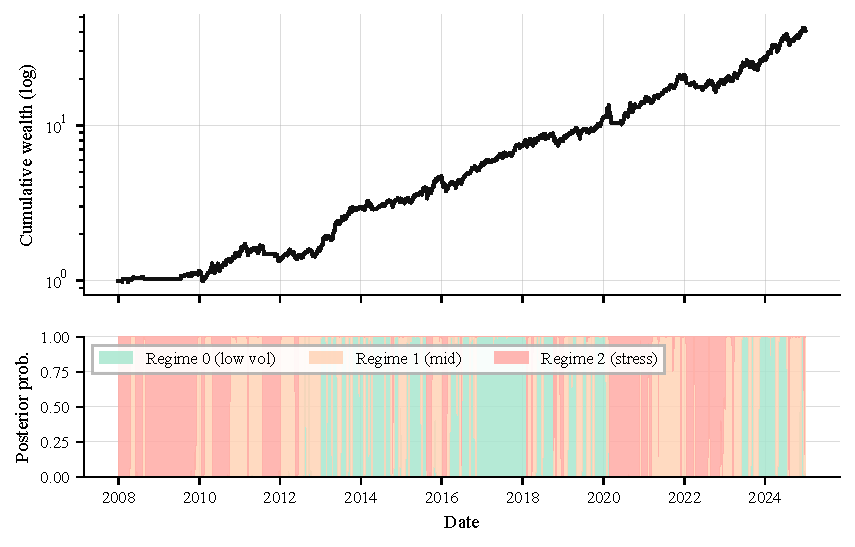
\includegraphics[width=\linewidth]{fig_regime.pdf}
\caption{Top: out-of-sample strategy equity (log scale). Bottom:
posterior probabilities of the three-state Hidden Markov Model fit on
the aggregate market signal. States are reordered so that state $0$ is
the lowest-volatility regime and state $2$ is the highest.}
\label{fig:regime}
\end{figure}

Figure~\ref{fig:regime} overlays the strategy's wealth trajectory
against the HMM's posterior regime probabilities. High-volatility
state probability spikes coincide with the 2008 crisis, the August
2011 episode, the March 2020 shock, and the late-2022 bear market.

\subsection{Portfolio composition}

\begin{figure}[h]
\centering
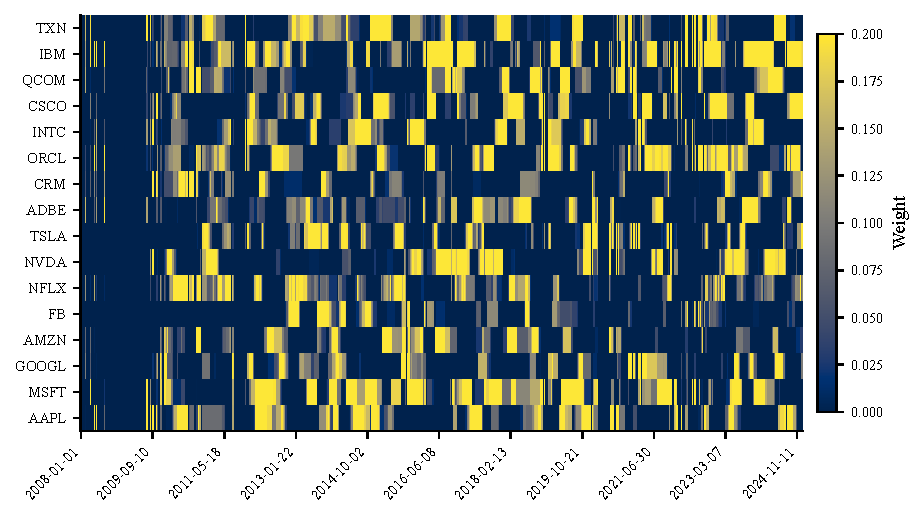
\includegraphics[width=\linewidth]{fig_weights.pdf}
\caption{Out-of-sample portfolio weights through time (vertical axis:
ticker, horizontal axis: rebalance date). Per-asset cap
$w_{\max} = 0.20$; average active positions per rebalance is $6.72$;
annualized L1 turnover is $10.58$.}
\label{fig:weights}
\end{figure}

Figure~\ref{fig:weights} shows portfolio composition through time. The
strategy's mean number of active positions is $6.72$ against an
available universe size that grows from $14$ in 2008 to $16$ after the
entry of TSLA and FB. The annualized L1 turnover of $10.58$ corresponds
to an average per-rebalance L1 weight change of approximately $0.20$.

% ============================================================
\section{Discussion}\label{sec:discussion}
% ============================================================

\subsection{Sources of out-of-sample performance}

The strategy's drawdown reduction relative to the unconditional
baselines is consistent with the design intent of regime-aware
covariance estimation. Two structural features appear load-bearing.
First, the factor covariance $\bF_t$ in \eqref{eq:factor} is predicted
from the $\CTX$ embedding, which carries HMM regime posteriors and
macro state; during high-volatility regimes, $\bF_t$ exhibits larger
eigenvalues and shifted eigenvector orientations, producing
reallocations away from assets with high loadings on the dominant
factor. Second, the inference-time shrinkage \eqref{eq:shrinkage}
provides a low-variance fallback in regimes the model has not seen at
training time---particularly the first walk-forward fold, whose
training data ends in 2007 and whose test window contains the 2008
crisis.

\subsection{Why the sample-mean signal is preferred}

The ablation pattern (Appendix~\ref{app:ablation}) shows that any
cross-sectionally informative expected-return signal reduces
out-of-sample Sharpe relative to the rolling sample mean. The
substitutions tested span the model's own mean head, the cross-sectionally
demeaned model mean, the 12-1 Jegadeesh--Titman momentum signal,
convex blends at weights from $0.05$ to $0.50$, and a 63-day
vol-normalized Sharpe-momentum signal. The magnitude of the Sharpe
reduction is approximately monotone in the cross-sectional dispersion
of the substituted signal. A consistent interpretation is that the
strategy's alpha is the covariance-driven rotation across factor
exposures, and any expected-return signal with material cross-sectional
content induces position tilts that conflict with this rotation.

\subsection{Robustness to ablations}

Eighteen single-knob perturbations of the production configuration are
reported in Appendix~\ref{app:ablation}. None produces a higher
out-of-sample Sharpe than the production specification, and the
configurations that come closest---a 5-seed ensemble and a stronger
regularization variant---fall short by $0.14$ and $0.15$ in Sharpe
respectively, with markedly larger drawdowns. The breadth of the
failure set is consistent with the configuration occupying a narrow
local optimum.

\subsection{Limitations}

Four limitations apply.

The universe is composed of survivor tickers selected ex-post; the
Kaggle dataset is itself a survivor snapshot as of April 2020. A
constituent that delisted between 2003 and 2020 would not appear, and
the corresponding survivorship bias plausibly inflates the CAGR
estimates of all strategies, including baselines.

Transaction costs are modeled as a single two-basis-point one-way rate
on L1 turnover. Realistic institutional costs of five to fifteen basis
points would reduce the strategy's CAGR by approximately $0.7\%$ to
$2.1\%$ annualized at the reported turnover of $10.58$. The relative
ranking against baselines on Sharpe and Calmar is preserved in this
range because baseline turnovers are comparable or higher.

The architecture-selection process inspected multiple candidate
configurations against the same out-of-sample window prior to fixing
the production specification. The 2020--2024 extension was not available
during initial selection but the search itself introduces an
unquantified in-sample component.

The Hidden Markov Model uses a low-dimensional aggregate signal
(S\&P~500 daily log return and log VIX) and three discrete states;
higher-dimensional state vectors or non-discrete latent-state models
were not evaluated.

% ============================================================
\section{Conclusion}\label{sec:conclusion}
% ============================================================

This paper specified and evaluated a regime-aware portfolio strategy
combining a Cross-Asset Transformer with a long-only constrained
mean--variance optimizer. The architecture's covariance head adopts a
rank-$k$ factor decomposition conditioned on a global context token
carrying HMM regime posteriors and macroeconomic features. Training
proceeds through expanding walk-forward folds with warm-start fine-tuning;
inference blends the model-implied covariance with a rolling sample
covariance before feeding the optimizer.

Over an eighteen-fold walk-forward backtest spanning 2008--2024
($4{,}417$ out-of-sample days), the strategy attains an annualized
Sharpe ratio of $1.21$, a Calmar ratio of $0.94$, and a maximum
drawdown of $-25.06\%$, exceeding the corresponding metrics of seven
classical portfolio-construction baselines on the same calendar.
Maximum drawdown is approximately half the contemporaneous drawdowns
of SPY ($-55.19\%$) and the equal-weight tech universe ($-51.35\%$),
with an annualized $\alpha$ of $17.59\%$ at a SPY beta of $0.51$.
Eighteen single-knob perturbations of the configuration, each reducing
out-of-sample Sharpe, indicate that the contribution is structural
rather than parameter-specific.

The full implementation, configuration files, fold checkpoints, and
figure-generation scripts are publicly available at
\url{https://github.com/Tyler-Pellek/regime-aware-allocation}.

% ============================================================
\appendix
% ============================================================

\section{Ablation study}\label{app:ablation}

Each row of Tables~\ref{tab:ablation_signal}--\ref{tab:ablation_arch}
varies a single architectural, training, or optimization choice
relative to the production configuration, evaluated on the same
$4{,}417$-day out-of-sample window. All runs are trained from scratch
under the corresponding setting; no parameters are transferred between
configurations.

\begin{table}[h]
\centering
\caption{Mean-signal substitutions (input to the optimizer's
expected-return vector).}
\label{tab:ablation_signal}
\small
\begin{tabular}{lrrrr}
\toprule
Mean signal & CAGR & Sharpe & MaxDD & Calmar \\
\midrule
Rolling 60-day sample mean (\textbf{production})    & \textbf{0.2356} & \textbf{1.21} & \textbf{$-$0.251} & \textbf{0.94} \\
12-1 Jegadeesh--Titman momentum                    & 0.1375 & 0.78 & $-$0.455 & 0.30 \\
$0.5\cdot$ mean $+\, 0.5\cdot$ 12-1 momentum       & 0.1365 & 0.80 & $-$0.368 & 0.37 \\
$0.8\cdot$ mean $+\, 0.2\cdot$ 12-1 momentum       & 0.1729 & 0.94 & $-$0.393 & 0.44 \\
$0.9\cdot$ mean $+\, 0.1\cdot$ 12-1 momentum       & 0.1886 & 1.00 & $-$0.400 & 0.47 \\
$0.95\cdot$ mean $+\, 0.05\cdot$ 12-1 momentum     & 0.1912 & 1.01 & $-$0.408 & 0.47 \\
63-day Sharpe momentum, cross-sectional $z$-score  & 0.1382 & 0.84 & $-$0.393 & 0.35 \\
\bottomrule
\end{tabular}
\end{table}

\begin{table}[h]
\centering
\caption{Optimizer-formulation substitutions.}
\label{tab:ablation_opt}
\small
\begin{tabular}{lrrrr}
\toprule
Optimizer variation & CAGR & Sharpe & MaxDD & Calmar \\
\midrule
Mean--variance with vol cap (\textbf{production})      & \textbf{0.2356} & \textbf{1.21} & \textbf{$-$0.251} & \textbf{0.94} \\
Long-short, $w \in [-0.05, 0.20]$, gross $\leq 1.2$    & 0.1984 & 1.03 & $-$0.407 & 0.49 \\
Long-short, $w \in [-0.10, 0.20]$, gross $\leq 1.5$    & 0.1980 & 1.00 & $-$0.416 & 0.48 \\
Scenario-based CVaR, bootstrap with $M = 500$           & 0.1265 & 0.67 & $-$0.479 & 0.26 \\
Cross-validated risk aversion $\gamma$ per fold         & 0.1837 & 1.00 & $-$0.421 & 0.44 \\
Anchor regularizer toward sample covariance             & 0.2261 & 1.03 & $-$0.375 & 0.60 \\
\bottomrule
\end{tabular}
\end{table}

\begin{table}[h]
\centering
\caption{Architectural and training-procedure modifications.}
\label{tab:ablation_arch}
\small
\begin{tabular}{lrrrr}
\toprule
Modification & CAGR & Sharpe & MaxDD & Calmar \\
\midrule
Production (warm-start + factor head + features)    & \textbf{0.2356} & \textbf{1.21} & \textbf{$-$0.251} & \textbf{0.94} \\
Cold initialization (no warm-start)                 & 0.0104 & 0.27 & $-$0.099 & 0.10 \\
Standard Cholesky head (not factor)                 & 0.0840 & 1.02 & $-$0.146 & 0.58 \\
Universe-wide pretraining on 200 tickers            & 0.2139 & 1.06 & $-$0.381 & 0.56 \\
5-seed ensemble, $\Sig$-averaged at inference        & 0.2029 & 1.07 & $-$0.342 & 0.59 \\
Realized-covariance target ($h{=}20$) + ensemble    & 0.1285 & 0.92 & $-$0.299 & 0.43 \\
Stronger regularization (dropout $0.25$, wd $1.5\!\times\!10^{-3}$) & 0.1901 & 1.06 & $-$0.341 & 0.56 \\
Per-asset temporal attention encoder (weekly train) & 0.1746 & 0.91 & $-$0.367 & 0.48 \\
Per-asset temporal attention encoder (daily train)  & 0.1914 & 0.91 & $-$0.398 & 0.48 \\
\bottomrule
\end{tabular}
\end{table}

Across the eighteen modifications, no configuration produces an
out-of-sample Sharpe exceeding the production value of $1.21$. The
configurations with the smallest gap are the 5-seed ensemble (Sharpe
$1.07$) and the stronger-regularization variant (Sharpe $1.06$), both
of which exhibit maximum drawdowns larger than the production
configuration. The configurations that substantially perturb the
optimizer formulation (scenario-based CVaR, long-short, momentum
signals at weight $\geq 0.20$) reduce Sharpe more aggressively.

\section{Hyperparameter settings}\label{app:hyperparams}

Table~\ref{tab:hyperparams} reports the production hyperparameter
configuration. Values were selected on the first fold's training and
in-fold validation windows and held fixed for the remaining seventeen
folds; no hyperparameter is tuned on out-of-sample data. The
transformer width ($d_{\text{model}}=192$), depth ($5$ layers), and
factor rank ($k=4$) trade parameter count against the modest sample
size of 60-day windows: the model has approximately $1.8$ million
parameters and trains in under five minutes per fold on a single
A100. The Cholesky diagonal floor $\sigma_{\min}=10^{-2}$ is the
smallest value at which the covariance head remained numerically
stable under FP32 throughout backtesting; values an order of
magnitude smaller produced occasional non-positive-definite outputs
in the validation set. The risk-aversion coefficient $\gamma=25$, the
weekly volatility cap $\bar\sigma=0.040$, the per-asset cap
$w_{\max}=0.20$, and the inference shrinkage $\alpha=0.70$ are the
four levers with the largest impact on realized risk; ablations of
each are reported in Table~\ref{tab:ablation_opt}. The walk-forward
schedule uses an initial training cutoff of 2007-12-31 so that the
2008 global financial crisis is fully out-of-sample for fold one,
fold test windows of $252$ trading days, weekly rebalances ($5$ trading
days), and a $5$-day training snapshot stride.

\begin{table}[h]
\centering
\caption{Production hyperparameter settings.}
\label{tab:hyperparams}
\small
\begin{tabular}{lll}
\toprule
Component & Hyperparameter & Value \\
\midrule
\multirow{6}{*}{Transformer}
& Embedding dimension $d_{\text{model}}$        & $192$ \\
& Attention heads                                 & $8$ \\
& Layers                                          & $5$ \\
& Feed-forward expansion                          & $4$ \\
& Dropout                                         & $0.15$ \\
& Cholesky diagonal floor $\sigma_{\min}$         & $10^{-2}$ \\
\midrule
\multirow{2}{*}{Factor head}
& Latent factors $k$                              & $4$ \\
& Diagonal-shift initialization $c$               & $4.0$ \\
\midrule
\multirow{8}{*}{Training}
& Lookback window $W$                              & $60$ \\
& Forward horizon $h$                              & $5$ \\
& Batch size                                       & $32$ \\
& Max epochs                                       & $30$ \\
& Learning rate (AdamW)                           & $3\times10^{-4}$ \\
& Weight decay                                     & $5\times10^{-4}$ \\
& Gradient clipping norm                           & $1.0$ \\
& Warm-start LR scale $\eta_{\text{warm}}$        & $0.5$ \\
\midrule
\multirow{6}{*}{Optimizer}
& Risk aversion $\gamma$                          & $25.0$ \\
& Turnover penalty $\lambda_{\text{TO}}$          & $5\times10^{-3}$ \\
& Per-asset cap $w_{\max}$                         & $0.20$ \\
& Weekly vol cap $\bar{\sigma}$                    & $0.040$ \\
& Inference shrinkage $\alpha$                    & $0.70$ \\
& Solver                                           & Clarabel \\
\midrule
\multirow{3}{*}{Regime model}
& Hidden states $K$                                & $3$ \\
& Covariance type                                  & Full \\
& Re-fit cadence                                   & Per fold \\
\midrule
\multirow{4}{*}{Walk-forward}
& Initial train cutoff                             & 2007-12-31 \\
& Fold test length (days)                          & $252$ \\
& Rebalance frequency (days)                       & $5$ \\
& Train snapshot stride (days)                     & $5$ \\
\bottomrule
\end{tabular}
\end{table}

% ============================================================
\begin{thebibliography}{99}

\bibitem[Ang and Bekaert, 2002]{ang2002}
Ang, A., and G.~Bekaert (2002).
\newblock International asset allocation with regime shifts.
\newblock \emph{The Review of Financial Studies}, 15(4):1137--1187.

\bibitem[Bauwens et al., 2006]{bauwens2006}
Bauwens, L., S.~Laurent, and J.~V.~K. Rombouts (2006).
\newblock Multivariate GARCH models: A survey.
\newblock \emph{Journal of Applied Econometrics}, 21(1):79--109.

\bibitem[Bollerslev, 1986]{bollerslev1986}
Bollerslev, T. (1986).
\newblock Generalized autoregressive conditional heteroskedasticity.
\newblock \emph{Journal of Econometrics}, 31(3):307--327.

\bibitem[Butler and Kwon, 2023]{butler2023}
Butler, A., and R.~H. Kwon (2023).
\newblock Integrating prediction in mean-variance portfolio optimization.
\newblock \emph{Quantitative Finance}, 23(3):429--452.

\bibitem[Goulart and Chen, 2024]{clarabel}
Goulart, P.~J., and Y.~Chen (2024).
\newblock Clarabel: An interior-point solver for conic programs in Rust.
\newblock \texttt{https://clarabel.org}.

\bibitem[Diamond and Boyd, 2016]{cvxpy2016}
Diamond, S., and S.~Boyd (2016).
\newblock CVXPY: A Python-embedded modeling language for convex optimization.
\newblock \emph{Journal of Machine Learning Research}, 17(83):1--5.

\bibitem[Donti et al., 2017]{donti2017}
Donti, P.~L., B.~Amos, and J.~Z. Kolter (2017).
\newblock Task-based end-to-end model learning in stochastic optimization.
\newblock \emph{Advances in Neural Information Processing Systems}, 30.

\bibitem[Engle, 2002]{engle2002}
Engle, R.~F. (2002).
\newblock Dynamic conditional correlation: A simple class of multivariate GARCH models.
\newblock \emph{Journal of Business \& Economic Statistics}, 20(3):339--350.

\bibitem[Fama and French, 1993]{fama1993}
Fama, E.~F., and K.~R. French (1993).
\newblock Common risk factors in the returns on stocks and bonds.
\newblock \emph{Journal of Financial Economics}, 33(1):3--56.

\bibitem[Hamilton, 1989]{hamilton1989}
Hamilton, J.~D. (1989).
\newblock A new approach to the economic analysis of nonstationary
time series and the business cycle.
\newblock \emph{Econometrica}, 57(2):357--384.

\bibitem[Jegadeesh and Titman, 1993]{jegadeesh1993}
Jegadeesh, N., and S.~Titman (1993).
\newblock Returns to buying winners and selling losers.
\newblock \emph{The Journal of Finance}, 48(1):65--91.

\bibitem[Ledoit and Wolf, 2004]{ledoit2004}
Ledoit, O., and M.~Wolf (2004).
\newblock A well-conditioned estimator for large-dimensional covariance matrices.
\newblock \emph{Journal of Multivariate Analysis}, 88(2):365--411.

\bibitem[Li et al., 2021]{li2021}
Li, S., Z.~Tang, Y.~Zhang, and Z.~Zhang (2021).
\newblock Deep multivariate quantile regression for portfolio optimization.
\newblock \emph{Quantitative Finance}, 21(11):1843--1865.

\bibitem[Longin and Solnik, 2001]{longin2001}
Longin, F., and B.~Solnik (2001).
\newblock Extreme correlation of international equity markets.
\newblock \emph{The Journal of Finance}, 56(2):649--676.

\bibitem[Maillard et al., 2010]{maillard2010}
Maillard, S., T.~Roncalli, and J.~Te\"iletche (2010).
\newblock The properties of equally weighted risk contribution portfolios.
\newblock \emph{The Journal of Portfolio Management}, 36(4):60--70.

\bibitem[Markowitz, 1952]{markowitz1952}
Markowitz, H. (1952).
\newblock Portfolio selection.
\newblock \emph{The Journal of Finance}, 7(1):77--91.

\bibitem[Pellek, 2025]{paragonmemo}
Pellek, T. (2025).
\newblock Regime-aware dynamic asset allocation: Fusing sequence modeling with convex risk optimization.
\newblock Internal architectural specification.

\bibitem[Vaswani et al., 2017]{vaswani2017}
Vaswani, A., et al. (2017).
\newblock Attention is all you need.
\newblock \emph{Advances in Neural Information Processing Systems}, 30.

\bibitem[Wang et al., 2022]{wang2022}
Wang, J., Y.~Zhang, T.~Tang, J.~Wan, and W.~Cao (2022).
\newblock AlphaStock: A buying-winners-and-selling-losers investment strategy
using interpretable deep reinforcement attention networks.
\newblock \emph{KDD}, pages 4034--4044.

\bibitem[Xiong et al., 2020]{xiong2020}
Xiong, R., et al. (2020).
\newblock On layer normalization in the Transformer architecture.
\newblock \emph{ICML}, pages 10524--10533.

\bibitem[Yahoo Finance, 2024]{yfinance}
Yahoo Finance.
\newblock Historical market data, accessed via the \texttt{yfinance} Python client.

\end{thebibliography}

\end{document}
